\documentclass[bachelor, german ]{hgbthesis}
%\usepackage{natbib}
\usepackage[utf8]{inputenc}
\usepackage{graphicx}
\usepackage[backend=biber]{biblatex}
\addbibresource{literatur.bib}
% \usepackage[a4paper,left=25mm,right=25mm,top=25mm,bottom=25mm]{geometry}
\usepackage{hgblistings}
\usepackage{color}

\begin{document}
\tableofcontents
\chapter{Einleitung}

\section{Motivation}
placeholder
\pagebreak

\section{Zielsetzung}
placeholder
\pagebreak

\chapter{Grundlagen}
\section{API}

Der Begriff API steht für Application Programming Interface (auf Deutsch Anwendungs-Programmier-Schnittstelle).
Die Grundlagen heutiger APIs wurden 1952 von David Wheeler, einem Informatikprofessor an der Universität Cambrigde, in einem Leitfaden verfasst.
Dieser Leitfaden beschreibt das Extrahieren einer Sub-Routinen-Bibliothek mit einheitlichem dokumentierten Zugriff. \cite{wheeler1952use}
Ira Cotton und Frank Greatorex erwähnten den Begriff erstmalig auf der Fall Joint Computer Con.\cite{cotton1968data}
Dabei erweiterten sie den Leitfaden von David Wheeler um einen wesentlichen Punkt: Der konzeptionellen Trennung der Schnittstelle und Implementierung der Sub-Routinen-Bibliothek.
Somit kann die Implementierung auf die die Schnittstelle zugreift ohne Einfluss auf die Benutzer ausgetauscht werden.\cite{kress2020graphql}

\begin{quote}
APIs sind wie User Interfaces - nur mit anderen Nutzern im Fokus. David Berlind \cite{berlind2017apis}
\end{quote}

APIs sind also wie UIs für die Interaktion mit Benutzern gedacht.
Der wesentliche Unterschied zwischen UI-Schnittstellen und einer API liegt aber an der Art der Nutzer die auf das Interface zugreifen.
Bei UIs spricht man von einem \textit{human-readable-interface}, das bedeutet das ein menschlicher User mit dem System interagiert.
Bei einer API spricht man von einem \textit{machine-readable-interface}, also von einer Schnittstelle die für die Kommunikation zwischen Maschinen gedacht ist.

\subsection{Abstraktes Beispiel API}
Ein abstraktes Beispiel für eine API wäre beispielsweise die Post. Angenommen eine Person will einen Brief an eine andere Person senden, um diese Person zum Essen einzuladen. Was passiert ist dann folgendes:
\begin{itemize}
 \item Person 1 verfasst eine Nachricht und packt diesen in einen Briefumschlag
 \item Der Briefumschlag wird mit einer Briefmarke und der Adresse des Empfängers und des Absenders versehen
 \item Der Brief wird nun an die Post übergeben
 \item Die Post kümmert sich um die Zustellung des Briefes
 \item Person 2 erhält den Brief
\end{itemize}

Damit dieser Zugriff der unterschiedlichen Systeme (hier Menschen) auf die Post funktioniert muss eine genaue Definition des Service vorliegen. Die genaue Spezifikation des Service ist dabei folgende:
\begin{itemize}
 \item Das zu versendende Objekt (Brief, Paket, etc.) muss an einem Sammelposten der Post abgegeben werden
 \item Das Objekt ist dabei mit einer Empfängeradresse und einer Absenderadresse zu versehen, zusätzlich muss eine Briefmarke gekauft werden
\end{itemize}
Das stellt die Art des Services dar und legt somit fest was über die API versendet wird. Zudem wird die Repräsentation der API definiert, also in welcher Form der Service im System des Servicenutzers integiert wird.
Der Briefkasten / Sammelposten ist dabei die eigentliche Schnittstelle - also die API. Die Zustellung ist dabei Implementierungsdetail, der Weg vom Sammelposten der Post über die Verteilerzentren und mit dem Briefträger zum Empfänger.
Dieses Implementierungsdetail kann beliebig angepasst werden, die Zustellung kann beispielsweise über den Land- oder Luftweg erfolgen. Der Benutzer welcher den Brief versendet hat ist davon nicht betroffen.

\section{REST-API}
REST steht für Representational State Transfer \cite{wheeler1952use}. REST ist dabei aber keine konkrete Technologie oder ein Standard. REST beschreibt einen Architekturstil welcher im Jahr 2000 von Roy Fielding konzipiert wurde.
Bei REST werden Daten als Ressourcen gesehen und in einem spezifischen Format übertragen. Ursprünglich wurde von Fielding dabei XML verwendet. XML wird aber in den letzten Jahren verstärkt durch JSON abgelöst.
\newline


Deswegen ist JSON besser als XML für den Austausch einfacher Daten mittels einer API geeignet:
\begin{itemize}
    \item JSON wurde speziell für den leichtgewichtigen Datenaustausch konzipiert.
    \item JSON ist schneller als XML
    \item JSON hat weniger Overhead als XML da XML deklarativ ist und somit wesentlich mehr Daten als JSON beinhaltet
\end{itemize}

Zum Vergleich hier ein Buch welches in JSON und XML repräsentiert wird:
\begin{JsCode}
{
    "isbn": "978-3551555557",
    "title": "Harry Potter und der Orden des Phönix",
    "releaseDate": "2003-11-15T00:00:00.000Z"
}
\end{JsCode}

\begin{XmlCode}
<book>
    <isbn name="isbn" type="string">978-3551555557</isbn>
    <title name="title" type="string">Harry Potter und der Orden des Phönix</title>
    <releaseDate name="isbn" type="dateTime">2003-11-15T00:00:00.000Z</releaseDate>
</book>
\end{XmlCode}

Wie in den obigen Code Beispielen ersichtlich produziert JSON (134 Bytes) wesentlich weniger Daten als XML(238 Bytes).
Man kann zusammengefasst also sagen, wenn es rein um die Datenübertragung geht, ist JSON deutlich leichtgewichtiger und damit auch performanter.

\subsection{REST-Bedingungen}
Die Begriffe Web und HTTP müssen von REST unterschieden werden, da REST lediglich einen Architekturstil beschreibt. Das Web hingegen besteht aus mehreren Architekturstilen und nutzt als Standargkommunikationsprotokoll HTTP. HTTP ist als
REST-konforme Implementierung zu erachten.
\newline


REST hat folgende architektonische Bedingungen:

\begin{enumerate}
    \item \textbf{Einheitliche Schnittstelle: }
    Jeder REST-Client der auf den Server zugreift muss auf dieselbe Art und Weise zugreifen.
    Dabei ist es egal ob der Client ein Browser, eine Desktop-Applikation oder eine mobile Anwendung ist.
    Dabei kommt hier HTTP mit der Verwendung einer URI - \textit{Unique Resource Identifier}, welche dann eine URL ist wie zum Beispiel: \textit{https://api.twitter.com}, zu tragen.
    Desweiteren müssen Anfragen autark sein - der Client überträgt alle Informationen, die der Server für die Abarbeitung der Anfrage benötigt, mit.
    Zudem wird die Implementierung von dem Service der sie zur Verfügung stellt entkoppelt, man kann also die Implementierung beliebig weiterentwickeln oder austauschen.
    \item \textbf{Client-Server Architektur: }
    Durch das Client-Server Prinzip werden verteilte Systeme beschrieben, die mittels netzwerkbasierter Kommunikation miteinander kommunizieren.
    In der REST-Architektur sind der Client und der Server klar voneinander abgetrennt.
    Damit ist es möglich beide Komponenten unabhängig voneinander weiterzuentwickeln, ohne dabei Einfluss auf die jeweils andere Kompnente zu haben
    \item \textbf{Zustandslosigkeit (Stateless): }
    Zustandlosigkeit bedeutet, dass der Client alle Informationen die der Server benötigt mitsendet.
    Das resultiert darin, dass der Server keine Overhad Daten des Clients speichern muss um zukünfige Anfragen abarbeiten zu können.
    Dadurch ist es auch möglich eine Lastverteilung (also mehrere Serverinstanzen nebeneinander laufen zu lassen) zu realisieren. Dies wiederum erleichtert die Skalierbarkeit des Servers.
    \item \textbf{Schichtsystem: }
    Geschichtete Systeme sind Systeme die aus mehreren hierarchischen angeordneten Schichten bestehen. Ein geschichtetes System wäre in .NET beispielsweise so umzusetzen:
    \begin{itemize}
        \item Controller (Leitet die Anfrage an die Logik weiter)
        \item Business-Logik (Setzt die geforderte Aktion um)
        \item Datenbankzugriff
    \end{itemize}
    Durch dieses Schichtsystem werden die Abhängikeiten im System reduziert und die Austauschbarkeit der einzelnen Komponenten erleichtert.
    \item \textbf{Zwischenspeicher (Cache): }
    Um wiederkehrende Anfragen performanter abwickeln zu können, kann dem Server mithilfe des \textit{Cache-Control-Headers} mitgeteilt werden, ob die angefragten Daten zwischengespeichert werden sollen.
    Zusätzlich muss definiert werden wielange dieser Cache gültig ist. Nach Ablauf der Gültigkeit werden die Daten erneut vom Server geladen.
    Durch das Zwischenspeichern von Daten wird die Performanz des Servers gesteigert. Ein Nachteil besteht dahingehend, dass dem Client womöglich nicht immer die aktuellsten Daten zur Verfügung stehen.
    \item \textbf{Code auf Anfrage: }
    Hierbei handelt es sich um eine optionale Bedingung, die Code-Snippets für die lokale Ausführung an den Client senden kann. Beispielsweise als JavaScript-Code innerhalb einer HTML-Antwort.
\end{enumerate}

\subsection{Kommunikation mit dem Server}
Die Kommunikation zwischen Server und Client wird bei einer RESTful-API mittels HTTP und dessen Methoden realisert.
Um CRUD (Create, Read, Update, Delete) Operationen auf Ressourcen abzusetzen werden folgende Methoden verwendet:
\begin{enumerate}
    \item \textbf{GET: }Wird als lesender Zugriff auf eine Ressource verwendet.
    \item \textbf{PUT: }Wird verwendet um eine Ressource zu aktualisieren.
    \item \textbf{POST: }Wird verwendet um eine neue Ressource zu erstellen.
    \item \textbf{DELETE: }Wird für das Löschen einer Ressource verwendet.
\end{enumerate}

Zusätzlich wird dem Client mittels HTTP-Statuscodes mitgeteilt ob die Anfrage erfolgreich war oder fehlgeschlagen ist. Beispielsweise werden hier Statuscodes angeführt die an den Client zurückgesendet werden:
\begin{itemize}
    \item \textbf{Erfolgreich:} 200
    \item \textbf{Anfrage fehlerhaft:} 400
    \item \textbf{Server interner Fehler:} 500
\end{itemize}

\section{GraphQL}
Die Informationen für dieses und das folgende Kapitel wurden aus diesen Quellen bezogen \cite{kress2020graphql, graphqlOnline, dgraphOnline, rakutenGraphQLVsRest}
\newline


2015 veröffentlichte Facebook unter der MIT-Lizenz GraphQL. GraphQL ist die Spezifikation einer plattformunabhängigen Query-Sprache. GraphQL dient als Übersetzer der Kommunikation zwischen Client und Server.
Die Kommunikation erfolgt wie bei REST über ein Request-Response-Schema.
Der wesentliche Unterschied zu REST-APIs besteht darin, dass GraphQL genau einen Endpunkt, anstatt für jede Ressource einen eigenen Endpunkt, zur Verfügung zu stellt.
Desweiteren werden nur POST-Anfragen von GraphQL akzeptiert, diese können lesend (Query) oder schreibend (Mutation) sein.

\subsection{Entwurfsprinzipien}
GraphQL definiert keine Implementierungsdetails sondern diese Entwurfsprinzipien:
\begin{enumerate}
    \item \textbf{Produktzentriert:}
    Die Anforderungen der Clients (Darstellung der Daten) stehen im Mittelpunkt. GraphQL bietet mit der Abfragesprache dem Client die Möglichkeit genau die Daten abzufragen, die er tatsächlich benötigt. Die Hierarchie der
    Abfrage wird dabei durch eine Menge ineinander geschachtelter Felder abgebildet.
    \item \textbf{Hierarchisch:}
    Jede Anfrage ist wie die Daten die er anfordert geformt.
    Das bedeutet, dass der Client die Daten genau in dem Format erhält wie in der Anfrage spezifiziert. Das ist ein intuitiver Weg für den Client um seine Datenanforderungen zu definieren.
    \item \textbf{Strenge Typisierung:}
    Jeder GraphQL-Service definiert ein für das System spezifisches Typ-System. Anfragen werden im Kontext dieses Typ-Systems ausgeführt.
    Mit Tools wie zum Beispiel GraphiQL kann man vor Ausführung der Anfrage sicherstellen, dass sie syntaktisch und semantisch korrekt sind.
    \item \textbf{Benutzerdefinierte Antwort:}
    Durch das Typ-System veröffentlicht der GraphQLService die Möglichkeiten, die ein Client hat um auf die dahinterliegenden Daten zuzugreifen.
    Der Client ist dafür verantwortlich genau zu spezifizieren wie er diese Möglichkeiten nutzen will.
    Bei einer normalen REST-API liefert ein Endpunkt jene Daten einer Ressource zurück welche vom Server definiert wurden.
    Bei GraphQL werden hingegen genau jene Daten einer Ressource zurückgegeben, die vom Client in seiner Anfrage definiert wurden.
    \item \textbf{Introspektion:}
    Das Typ-System eines GraphQL-Services kann direkt mit der GraphQL-Abfragesprache abgefragt werden. Diese Abfragen werden für die Erstellung von Tools für GraphQL benötigt.
\end{enumerate}

\section{GraphQL vs. REST}
\subsection{Endpunkte}
Eine REST-API bietet für jede Ressource verschiedene Endpunkte an um CRUD Operationen für die jeweilige Ressource auszuführen. GraphQL hingegen bietet nur einen
Endpunkt. An diesem kann der Client eine Abfrage mit einer Query oder einer Mutation senden um auf die jeweilige Ressource zuzugreifen.

\subsection{Over-fetching und Under-fetching}
Als Over-fetching wird das Laden von zuvielen oder nicht benötigten Daten bezeichnet.
Under-fetching bedeutet, dass man mehr Daten benötigt als der Server dem Client zurückgibt. Dieses Problem tritt bei REST-APIs auf die viele verschiedene Clients mit Daten versorgen müssen (beispielsweise eine Desktop-Applikation, eine Mobile-Anwendung
und ein Web-Client). Grundsätzlich wollen alle drei Clients diesselbe Ressourcen abfragen, mit dem Unterschied, dass die Mobile Anwendung beispielsweise nicht alle Daten
benötigt. Die Desktop-Applikation möchte aber alle Daten einer Ressource bekommen
um diese darzustellen. Eine Lösung dafür wäre beispielsweise einen Endpunkt für jeden
Client zu definieren um die für ihn benötigen Daten zur Verfügung zu stellen. Dies resultiert aber in mehr Programmieraufwand und damit auch einer höheren Komplexität
der Anwendung.
\newline

Dieses Problem kann bei GraphQL nicht auftreten da der Client in seiner Anfrage genau die Daten definiert die er braucht.

\subsection{Was ist für welches Szenario besser geeignet?}
Möchte man ein System entwickeln auf welches verschiedene Clients (die verschiedene Anforderungen an die Ressourcen haben) zugreifen, dann ist GraphQL die bessere
Wahl. Würde man dieses System mit einer REST-API umsetzen, müsste man entweder
Probleme mit Under-fetching und Over-fetching in Kauf nehmen, oder für jeden Client eine eigene Route definieren. GraphQL ist in diesem Szenario deshalb als besser zu
erachten, weil man sich mit der einmaligen Implementierung des Schemas zusätzliche
Routendefinitionen erspart. Dadurch hat man automatisch weniger Entwicklungsaufwand und generell weniger Komplexität.
\newline


Verfolgt man aber das Ziel ein System zu entwickeln, welches keine komplexen Daten enthält und beispielsweise nur mit einem Web-Client kommuniziert, ist eine REST-API die bessere Wahl.

\chapter{GraphQL}

\section{Interfaces}

\section{Input Typen}

\section{Typ System Schema Definition}

Im GraphQL-Schema werden die Ressourcen, die Relationen zwischen den Ressourcen, die lesenden und schreibenden Operationsmöglichkeiten auf die Ressourcen definiert.
\newline

Es wird die genaue Datenstruktur definiert mit welcher ein eingehender Request validiert wird.
Entspricht die im Request enthaltene Query oder Mutation dem Schema so wird der Inhalt an die Implementierung des Schemas für die Verarbeitung weitergeleitet.
GraphQL zerlegt dafür die Query oder Mutation und gibt sie an den jeweiligen Resolver weiter. Seite 57 und 58

\section{Grundlegendes Schema}
Das grundlegende Schema bezieht sich auf die Ressourcen und die Relationen dieser Ressourcen zueinander.

\begin{JsCode}
type Book {
    id: Int!
    title: String
    authors: [Author]
}
    
type Author {
    id: Int!
    firstName: String
    lastName: String
    books: [Book]
}
\end{JsCode}

Im oben angeführten Codebeispiel werden die beiden Objekttypen Author und Book definiert.
Die Ressource Book enthält dabei die Felder id und title. Desweiteren enthält Book eine Liste von Authoren.
Die Ressource Author enthält die Felder id, firstName und lastName.
Außerdem enthält Author eine Liste von Büchern die der Autor geschrieben hat.
Im Beispiel gilt zu beachten, dass eine Ressource mit dem Schlüsselwort \textit{type} versehen ist.
Zudem sind die Properties der Ressource immer nach dem Schema <name>: <Datentyp> gegliedert.
Der Datentyp ist dabei entweder ein Objekt, eine Liste von Objekten oder ein skalarer Datentyp.
Im Schema werden Relationen von Objekten nicht durch eine Schachtelung dieser in einem einzigen Objekt definiert.
Bei komplexeren Graphen würde dies zu einer kaum zu lesenden oder adaptierbaren Schemadefinition führen.
Das Schema besteht somit aus einzelnen, geschlossenen Objekttyp-Definitionen, die einander oder aber ihre Felder referenzieren. Seite 58 und 59
Ist ein Feld mit ! deklariert so darf dieses nicht null sein.


\section{Parameter}

\section{Skalare}

Wenn man das Schema als Baumstruktur betrachtet so sind die referenzierten Objekte Verzweigungen des Baumes.
Die Blätter am Ende des Baumes enthalten die eigentlichen Daten.
Die Astverzweigungen sind wichtig, denn sie sind die Referenzen die zu den anderen Objekten verweisen.
Ein Datentyp der nicht mehr weiter vereinfach bar ist wird wie in anderen Programmiersprachen Skalar-Typ genannt.
Bereits vordefinierte Skalar-Typen von GraphQL sind:

\begin{enumerate}
    \item Boolean
    \item Float
    \item Int
    \item String
    \item ID
\end{enumerate}
In den meisten sprachspezifischen Implementierungen ist es möglich eigene Skalar-Typen zu definieren. Diese werden verwendet um beispielsweise verschiedene Datumsformate darzustellen.

\section{Querys}

GraphQL erlaubt es den Clients lesend auf die Ressourcen zuzugreifen und genau jene Daten abzufragen welche er benötigt.
Als Ergebnis auf eine Anfrage werden die Daten genau in dem Format zurückgegeben in welcher die Anfrage erfolgt ist.
Dafür bietet GraphQL den Eingangspunkt hinter dem sich das komplette zuvor definierte Graphen Schema befindet.
Um nun auf die Daten zugreifen zu können, muss an den Endpunkt ein in der GraphQL Query Language definiertes Objekt mit den Feldern des Graphen, übergeben werden.
Um nun auf die im Schema definierten Ressourcen lesend zugreifen zu können muss das Schema um Querys erweitert werden. 

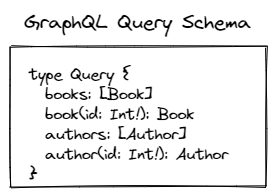
\includegraphics{pics/GraphQL_Query_Schema.png}

\subsection{Designempfehlungen}

placeholder
\pagebreak

\subsection{Verschachtelte Querys}

\subsection{Variablen}

placeholder
\pagebreak

\subsection{Fragmentierung}

\subsection{Aliase}

placeholder
\pagebreak

\section{Mutationen}

\subsection{Designempfehlungen}

placeholder
\pagebreak

\section{Bekannte Probleme}

\subsection{Authentifizierung, Autorisierung und Rollenmanagement}

placeholder
\pagebreak

\subsection{1 + n Problem}

\subsection{Subscriptions}

placeholder
\pagebreak

placeholder
\pagebreak

\subsection{Fehlermanagement}

placeholder
\pagebreak

\subsection{Pagination}

\subsection{Caching}

placeholder
\pagebreak

\chapter{Entwicklung}

\section{Anwendungsszenario}

\section{Architektur}

placeholder
\pagebreak

placeholder
\pagebreak

\section{Entwurf Schema}

placeholder
\pagebreak

\section{Umsetzung GraphQL mit .NET}

\subsection{Verwendete Bibliotheken}

placeholder
\pagebreak

\subsection{Entity Framework}

placeholder
\pagebreak

placeholder
\pagebreak

\subsection{Umsetzung Authentifizierung, Autorisierung, Rollenmanagement}

placeholder
\pagebreak

\subsection{Umsetzung Subscriptions}

placeholder
\pagebreak

\subsection{Umsetzung 1 + n Problem}

placeholder
\pagebreak

\subsection{Umsetzung Pagination}

\chapter{Conclusio}

\section{Fazit}

\section{Ausblick}

\printbibliography


\end{document}
